\section{Performance Evaluation}

In this section, we perform a performance evaluation of our proposal mechanism using a Netronome SmartNIC. We start by describing our environment setup, followed by discussing the results.

\subsection{Environment Setup and Baseline Comparison}

\noindent\textbf{Setup.} Our environment setup consists of three high-end servers. Each server has an Intel Xeon 4214R processor with 32 GB RAM. One server is our Device Under Test (DUT) -- i.e., the server in which our solution (i.e., P4 program) is loaded -- and the other two are used for traffic generation. All servers have a Netronome SmartNIC Agilio CX 10 Gbit/s network device with two network interfaces, which are physically connected (i.e., each traffic generator is connected to the DUT directly). 
%
We use MoonGen\cite{moongen} as our DPDK\footnote{\url{https://www.dpdk.org/}} traffic generator. We instruct MoonGen using the Netronome Packet Generator\footnote{\url{https://github.com/emmericp/MoonGen/tree/master/examples/netronome-packetgen}}. In our experiments, we send 64B IPv4 packets at line rate (i.e., 10Gbit/s) with random source and destination prefixes. One of the traffic generator servers is used to send foreground network traffic, while the second is used to inject abrupt network traffic from time to time. This abrupt network traffic is generated with MoonGen to lead to a congested scenario. The experiment is run through 105 seconds, divided by time slots/epochs of 15 seconds each. We sent network traffic bursts in the following slots: 2\textit{nd} (15s-30s), 4\textit{th} (45s-60s), 6\textit{th} (75s-90s). In our experiments, the SmartNIC Netronome acts simultaneously as an INT transit and an INT sink. First, it collects internal data plane metrics such as packet processing time and packet size (i.e., set $M'$). Then, we assume that both metrics are weighted equally (i.e., $w_1 = w_2$) for calculating $A_p$, $A_w$, and $A_e$. We varied the window size $W$ from $2^{20}$ to $2^{23}$ packets. Also, the parameters $\alpha$ in $A_e$ varies from $0.1$ to $0.9$. Our solution is compiled using the Netronome's P4 compiler. The compiled code is statically assigned to a single micro engine (ME) inside the SmartNIC. This is done as there are some limitations on the Netronome's Mutex implementation when using different memories hierarchies (i.e., different from the ones inside the ME). All experiments were run at least 30 times to ensure a confidence level higher than 90\%. \\

\noindent\textbf{Baseline.} We compare our \texttt{ETA} approach against the Full INT procedure and a fixed threshold one. In the former, all INT data are reported to the INT collector, while in the latter we use a constant value as the threshold. This constant value is obtained by calculating the average of all collected INT data in an offline manner. Our codes are publicly available\footnote{url{https://github.com/canofre/mestrado/}} in order to foster reproducibility.

\begin{figure}[!htb]
\centering
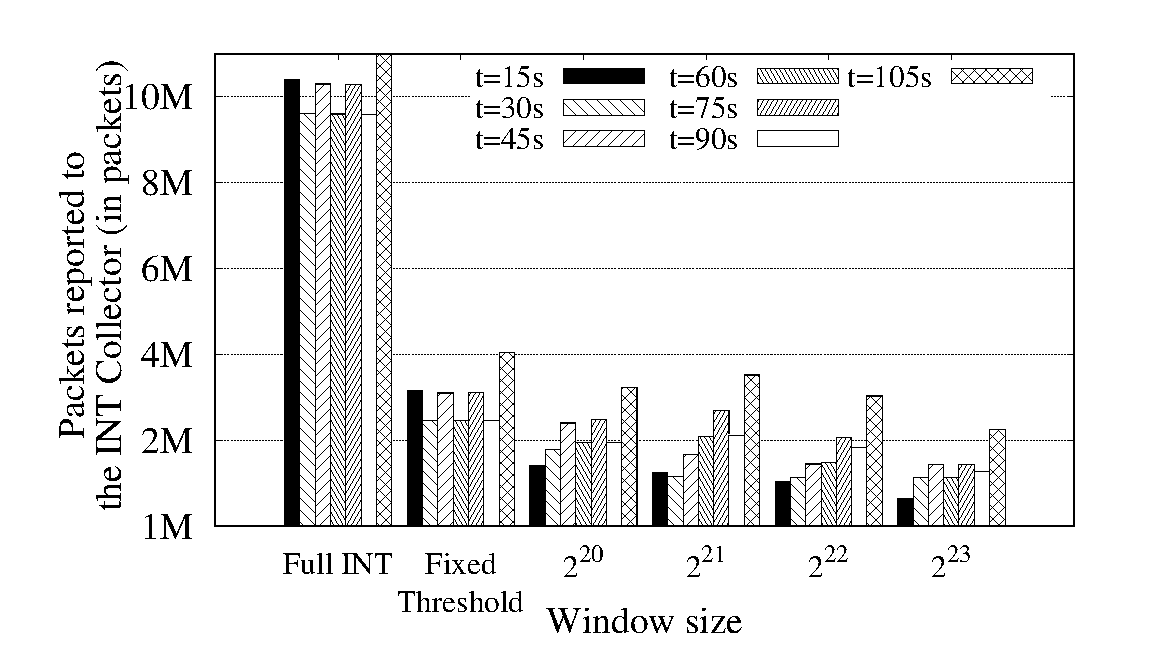
\includegraphics[scale=0.4]{results/g1a.eps}
\caption{Number of packets reported to an INT Collector.} 
\label{fig-results1}
\end{figure}

\subsection{Results}

\noindent \textbf{Number of packets sent to the INT Collector.} We start by analyzing the number of packets that have been sent to an INT Collector in a given window $W$ (Figure~\ref{fig-results1}). For this experiment, we consider that $\alpha = 0.1$ (we later analyzed its impact). We observe that our approach outperforms the Full INT and Fixed-Threshold procedures in terms of packets reported by a factor of 16$X$ and 5$X$, respectively. The main reason consists of the dynamic adjustment made in the threshold value over time. Further, we also observe that our approach decreases the number of reported packets as the size of the windows $W$ increases. For instance, we note 43$\%$ less network traffic being reported using a windows $W=2^{23}$ than $W=2^{20}$. With larger window size, our metrics $A_w$ tends to be smoother over time and less impacted by abrupt changes in the data plane metrics. Last, we also note a saw-tooth behavior between bars (e.g., $W=2^{30}$), which represents the effect of sending packet bursts in a given time interval. The larger is the window size, the less is the saw-tooth behavior observed.\\ 



\noindent \textbf{Impact of the window size on the computed average $A_e$.} Next, we evaluate how the average $A_e$ computed by the data plane evolves considering different window sizes (from $2^{20}$ to $2^{23}$). Figure~\ref{fig-result2} illustrates the behavior when setting $\alpha = 0.2$. When the window size is small (e.g., $2^{20}$), the average $A_e$ increases over time until reaching a stable value. On the contrary, larger windows tend to decrease the average $A_e$ value over time until reaching a similar stable value. With larger windows (i.e., $2^{22}$ and $2^{23}$), the summation made before computing $A_e$ within an epoch encompasses the periods where network bursts are sent. Therefore, it ends up increasing its initial value in comparison to small windows. Further, we also note that the value found in the stability tends to be more uniform in this case.\\ % with $\alpha = 0.2$ (i.e., we give importance of 0.8 to the historical behavior).\\  

\begin{figure}[!t]
\centering
%\subfigure[$\alpha = 0.1$]{
            %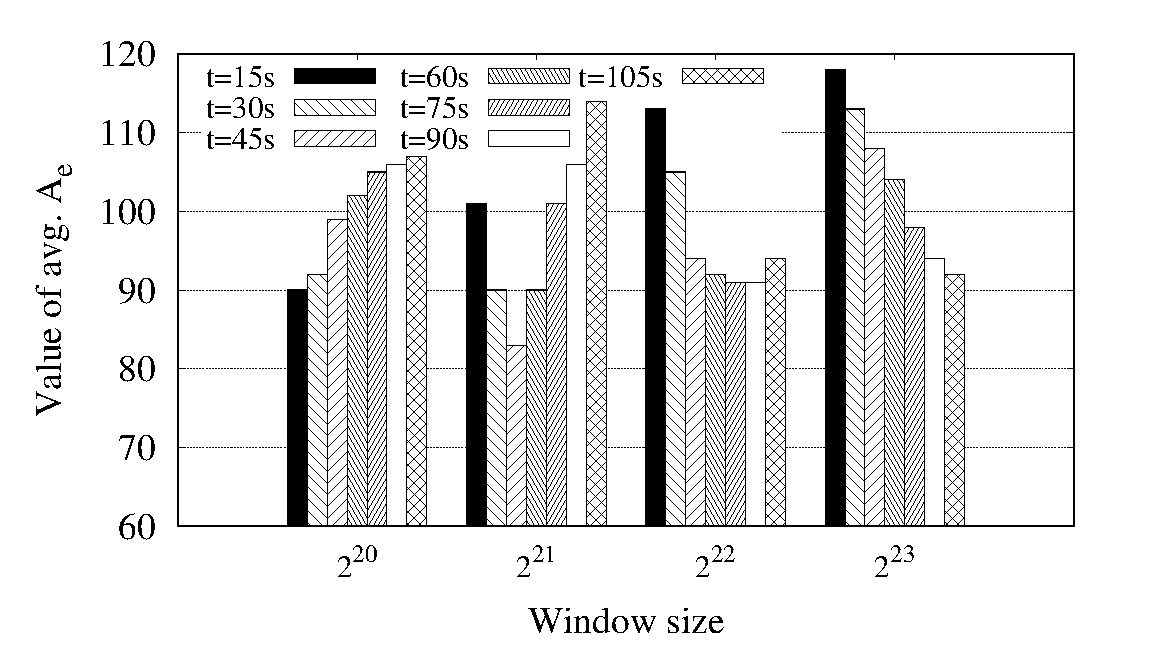
\includegraphics[scale=0.26]{results/g4a.eps}
            %\label{fig-g4-a}
        %}
%\subfigure[$\alpha = 0.2$]{
            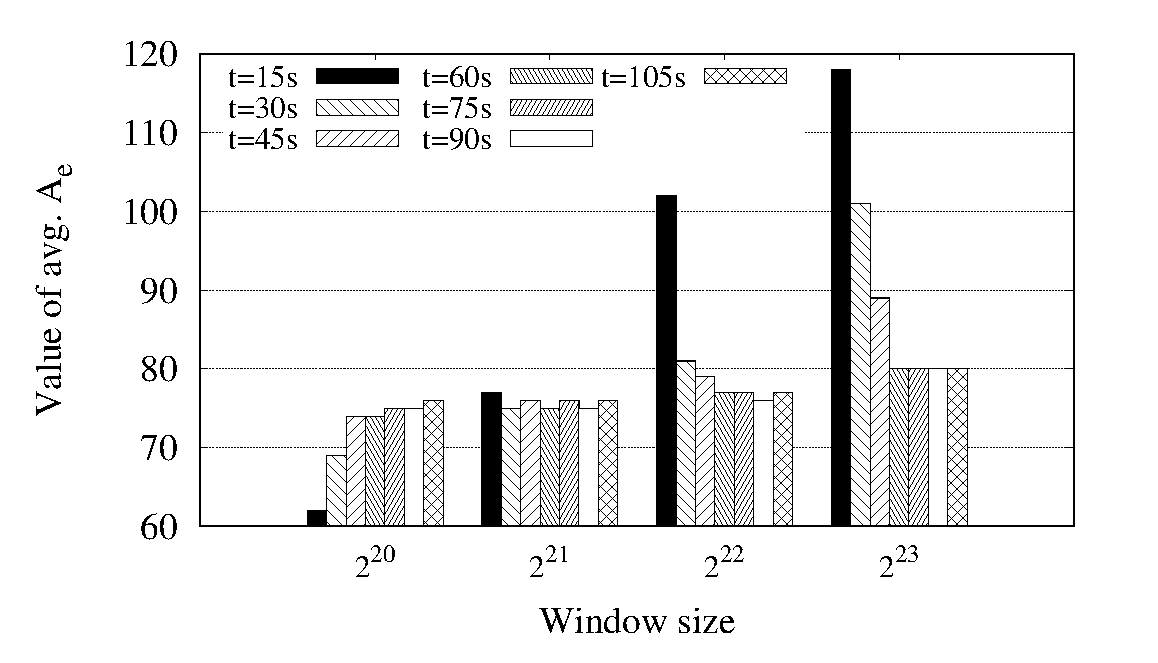
\includegraphics[scale=0.35]{results/g4b.eps}
    
   %     }
\caption{Impact of window size on the average $A_e$ with $\alpha = 0.2$}
  \label{fig-result2}
\end{figure}

\noindent \textbf{Impact of fine-tuning the parameters on the computed average $A_e$.} We analyzed how the $A_e$ evolves varying $\alpha$ from 0.1 to 0.9. For this experiment, we set the window size to $W = 2^{20}$. Note that higher values assigned to $\alpha$ tend to prioritize the behavior observed in the last time window (i.e., $A_w$), while lower values prioritize the historical behavior observed over time (i.e., $A_e$). As we can observe in Figure~\ref{fig-results3}, the higher the $\alpha$ values the higher the average $A_e$ gets over time. In this case, network traffic bursts change data plane metrics (e.g., in-network processing time) and then propagate such values' increases with more intensity to the following-up windows. In turn, lower values of $\alpha$ tend to prioritize the historical behavior and, therefore, the obtained values of $A_e$ are less susceptible to short network traffic variations.\\

\begin{figure}[!htb]
\centering
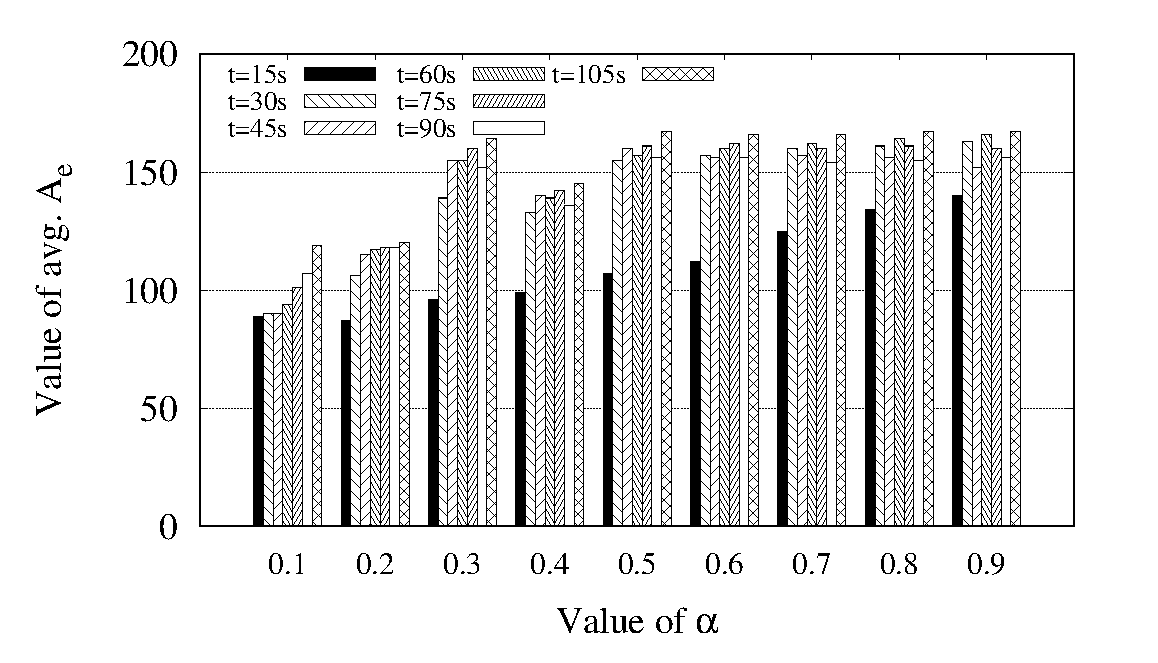
\includegraphics[scale=0.35]{results/g3.eps}
\caption{Impact of the fine-tuning of $\alpha$ on the computed average $A_e$ considering $W=2^{20}$.}
\label{fig-results3}
\end{figure}

\noindent \textbf{Impact on packet processing latency and throughput.} Last, we evaluate the impact of our approach in terms of packet processing and latency when processing packets in the data plane. First, Figure~\ref{fig-g5-a} depicts the achieved throughput in packets per second. Our approach is able to outperform the Full INT strategy and the Fixed Threshold by 50\% and by 10\%, respectively. However, when compared to the Basic Forward -- i.e., the same P4 code without any add-on -- our approach is limited to run at most 60\% of the maximum throughput. This occurs mostly because our approach demands more processing power and locks (due to mutex usage) and our approach is limited to running in a single ME (with 8 threads). In turn, Figure~\ref{fig-g5-b} illustrates the incurred data plane latency. We measured the latency as the difference between the ingress and egress timestamps inside the data plane. As we observe, our proposed approach adds around 60ns -- that is,  1.53X higher than the Basic Forwarding approach. In turn, the Full INT and the Fixed Threshold  approaches add 2.34X and 2.52X, respectively. 

\begin{figure}[!tb]
\centering
\subfigure[Measured throughput.]{
            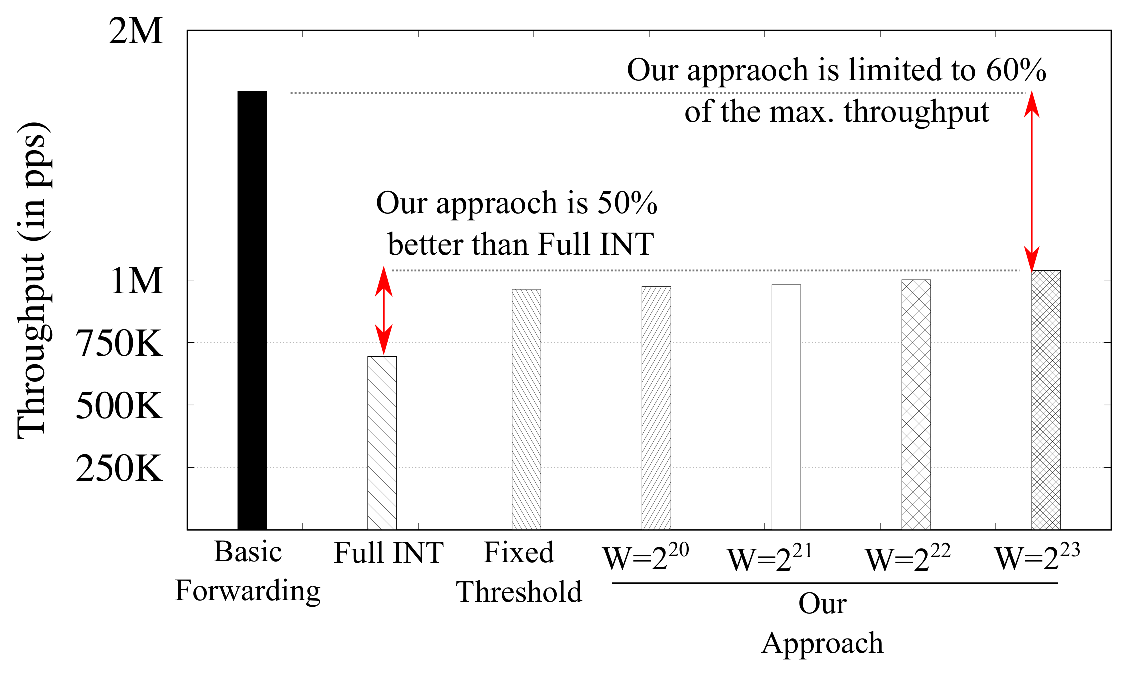
\includegraphics[scale=0.27]{results/g5-edited.eps}
            \label{fig-g5-a}
        }
\subfigure[Measured packet latency.]{
            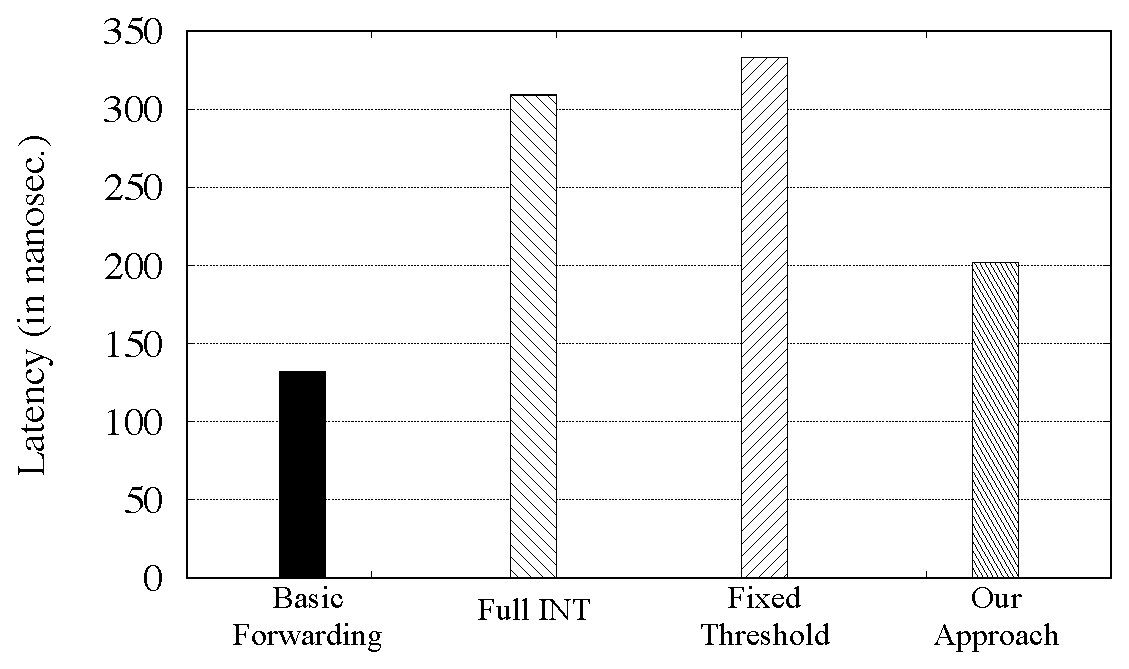
\includegraphics[scale=0.27]{results/g2.eps}
            \label{fig-g5-b}
        }
\caption{Impact of Throughput and Latency of our proposed approach.}
  \label{fig5}
\end{figure}



